\documentclass[lettersize,journal]{IEEEtran}
\usepackage{amsmath,amsfonts}
\usepackage{array}
\usepackage{textcomp}
\usepackage{stfloats}
\usepackage{url}
\usepackage{verbatim}
\usepackage{graphicx}
\usepackage{cite}
\usepackage{xcolor}
\usepackage{standalone}
\usepackage{wrapfig}
\usepackage{booktabs}
\usepackage{tikz}
\usetikzlibrary{shapes.geometric, shapes.misc, positioning,
                decorations.pathreplacing, arrows.meta, calc}
% Colors retained for potential use in other figures
\definecolor{factorfill}{RGB}{255,236,179}   % light amber
\definecolor{factordraw}{RGB}{191,127,0}     % dark amber
\newcommand{\todo}[1]{\textcolor{red}{[TODO: #1]}}
\newcommand{\Impl}[1]{\textsc{#1}}
\hyphenation{op-tical net-works semi-conduc-tor IEEE-Xplore}

\begin{document}

\title{Revisiting Prior Vehicle-Dynamics-Based Drowsy Driving Detection Methods
       Under Controlled Domain and Class Imbalance Conditions}

\author{Yutaro~Nakagama,
Daisuke~Ishii,~\IEEEmembership{Member,~IEEE,} and~Kazuki~Yoshizoe
\thanks{Manuscript received XXXX XX, 2026; revised XXXX XX, 2026.}%
\thanks{Y.~Nakagama and D.~Ishii are with the School of Information Science, Japan Advanced Institute of Science and Technology (JAIST), Nomi, Ishikawa 923-1292, Japan (e-mail: ynakagama@jaist.ac.jp; dsksh@jaist.ac.jp).}%
\thanks{K.~Yoshizoe is with the Research Institute for Information Technology, Kyushu University, Fukuoka 819-0395, Japan (e-mail: yoshizoe@cc.kyushu-u.ac.jp).}}

\markboth{IEEE Transactions on Intelligent Vehicles,~Vol.~XX, No.~XX, XXXX~2026}%
{Nakagama \MakeLowercase{\textit{et al.}}: Revisiting Prior Vehicle-Dynamics-Based DDD Methods}

\maketitle

\begin{abstract}
Prior vehicle-dynamics-based drowsy driving detection (DDD) studies established a common evaluation framework and found that a random forest (RF) outperforms three established methods---\Impl{SvmA} (Arefnezhad et~al.), \Impl{SvmW} (Zhao et~al.), and \Impl{Lstm} (Wang et~al.)---on a public 87-subject simulator dataset, while identifying domain shift and class imbalance as uncontrolled threats to validity~\cite{nakagama2025iv}.
A companion factorial experiment quantified these effects and demonstrated that within-domain training together with subject-wise oversampling (SW-SMOTE) raises RF's AUROC to 0.890 compared with 0.85 in the uncontrolled setting~\cite{nakagama2026tiv}.
This paper reports Experiment~3: we re-evaluate \Impl{SvmA}, \Impl{SvmW}, and \Impl{Lstm} under the same within-domain, imbalance-aware conditions using the identical experimental framework.
Three distinct failure modes emerge under controlled evaluation.
First, \Impl{SvmW} partially responds to rebalancing---best AUROC = 0.556, F2 = 0.347 with random under-sampling (RUS) at $r = 0.5$---but remains far below RF at 0.890.
Second, \Impl{SvmA} degenerates to a near-random predictor (AUROC $\approx$ 0.50) regardless of rebalancing strategy, revealing a collapse in the PSO-based adaptive feature selection.
Third, \Impl{Lstm} exhibits persistent positive-class bias (recall $\approx$ 0.98, F2 $\approx$ 0.92, best AUROC $\approx$ 0.82 for in-domain training with SW-SMOTE), showing genuine but limited discrimination (AUROC 0.82 vs.\ 0.890 for RF) while appearing deceptively strong on F2.
These findings confirm that RF's advantage is genuine: the controlled AUROC gap between RF and the best discriminating prior method (\Impl{SvmW}: AUROC 0.556) is 0.334, growing from the uncontrolled setting, while even the best-performing prior method by AUROC (\Impl{Lstm}: 0.82) remains 0.07 below RF under its best conditions.
Method-specific failure mode analysis reveals that ANFIS-based feature selection and event-based labeling are the primary failure sources, and provides concrete diagnostic criteria to guide future method development.
\end{abstract}

\begin{IEEEkeywords}
Drowsy driving detection, vehicle dynamics, random forest, class imbalance, domain shift, SMOTE, method comparison, reproducibility.
\end{IEEEkeywords}

%% ====================================================================
\section{Introduction}
\label{sec:intro}

\IEEEPARstart{D}{rowsy} driving is a leading cause of traffic accidents worldwide, accounting for an estimated 15--20\% of road fatalities~\cite{who2018}.
Vehicle-dynamics-based drowsy driving detection (DDD) offers a non-intrusive and practical approach by monitoring signals such as steering angle, lateral acceleration, and lane offset without requiring sensors attached to the driver~\cite{fu2024,fonseca2025}.
A growing body of work has reported high performance on this approach, with accuracy and AUC values reaching 90--98\%~\cite{arefnezhad2019,zhao2012,wang2022}, suggesting the problem may be close to solved.

Two recent studies from our group challenge this optimism and motivate the present work.
The first~\cite{nakagama2025iv} implemented three representative prior methods---\Impl{SvmA}~\cite{arefnezhad2019}, \Impl{SvmW}~\cite{zhao2012}, and \Impl{Lstm}~\cite{wang2022}---in a common framework on a public 87-subject driving simulator dataset~\cite{aygun2024} and compared their performance against a simple RF baseline under a standardized evaluation protocol.
That comparison found significant discrepancies from the originally reported values and established RF as the strongest method (AUROC = 0.85, accuracy = 88\%).
However, the comparison used a uniform evaluation protocol that did not separately account for two known data-quality challenges: \emph{class imbalance}, because drowsy episodes are rare in driving data, and \emph{domain shift}, because driving behavior varies across drivers.
Both factors were listed as threats to validity but were not controlled.

The second study~\cite{nakagama2026tiv} addressed this gap by constructing a four-factor full-factorial experiment on the same 87-subject dataset, varying distance metric~($D$), domain membership~($G$), training mode~($M$), and rebalancing strategy~($R$).
Sobol--Hoeffding variance decomposition over 1{,}512 RF evaluations revealed that training mode and rebalancing together account for $\geq$93\% of systematic performance variance, with a strong $R \times M$ interaction.
Specifically, within-domain training with subject-wise SMOTE (SW-SMOTE) at $r = 0.1$ yielded AUROC = 0.890, F2 = 0.559, and AUPRC = 0.617---significantly outperforming the uncontrolled baseline (AUROC = 0.684).
These results establish a principled set of best-practice conditions for vehicle-dynamics-based DDD.

A natural and important question then arises: \emph{do the conclusions of the prior comparison study hold when the same best-practice conditions are applied to the prior methods?}
If the prior methods were simply disadvantaged by the uncontrolled evaluation protocol, their performance under controlled conditions might be competitive with RF.
Conversely, if RF's advantage persists or grows under controlled conditions, this would provide strong evidence that it stems from a genuine method-level difference rather than an artifact of evaluation setup.
Furthermore, observing prior method behavior under controlled conditions may reveal failure modes that were masked in the uncontrolled setting.

To address these questions, this paper presents Experiment~3, in which we apply the evaluation framework of~\cite{nakagama2026tiv} to \Impl{SvmA}, \Impl{SvmW}, and \Impl{Lstm}.
Concretely, all three methods are trained and evaluated in within-domain mode with the full set of rebalancing strategies (baseline, RUS, SMOTE, SW-SMOTE at $r \in \{0.1, 0.5\}$) across three domain-partition distance metrics and both domain groups, over 15 random seeds (1{,}890 total evaluations across three prior models).

The main contributions of this paper are:
\begin{enumerate}
\item We systematically re-evaluate three published vehicle-dynamics-based DDD methods under the controlled domain and imbalance conditions identified in~\cite{nakagama2026tiv}, enabling a direct apples-to-apples comparison with RF.

\item We show that controlled evaluation exposes three distinct and interpretable method-level failure modes: (i)~PSO-based adaptive feature selection collapses to a trivial predictor in \Impl{SvmA}; (ii)~LSTM training with DRT-based labels under within-domain partitioning induces persistent positive-class bias in \Impl{Lstm} (recall $\approx$ 0.98, FP rate $\approx$ 88\% on alert windows); and (iii)~\Impl{SvmW} partially responds to rebalancing but remains substantially below RF.

\item We demonstrate that RF's advantage from~\cite{nakagama2025iv} is genuine: the controlled AUROC gap between RF and the best prior method by genuine discrimination (\Impl{SvmW}: 0.556) is 0.334; even the highest-AUROC prior method (\Impl{Lstm}: 0.821 in-domain) remains 0.069 below RF (0.890), with F2 driven by positive-class bias rather than balanced detection.
\end{enumerate}

The remainder of this paper is organized as follows.
Section~\ref{sec:related} reviews related work.
Section~\ref{sec:formulation} formalizes the DDD task and defines the three prior methods.
Section~\ref{sec:framework} describes the experimental framework, including common settings and the prior method implementations.
Section~\ref{sec:results} reports experimental results.
Section~\ref{sec:discussion} discusses the findings and their implications.
Section~\ref{sec:conclusion} concludes.

%% ====================================================================
\section{Related Work}
\label{sec:related}

\subsection{Vehicle-Dynamics-Based Drowsy Driving Detection}
Vehicle dynamics signals---steering wheel angle, lateral acceleration, and lane position---are widely used for DDD because they enable non-intrusive monitoring without physiological sensors attached to the driver~\cite{fu2024,fonseca2025,alquraishi2024,perkins2022}.
Among the methods evaluated in this paper,
Arefnezhad et~al.~\cite{arefnezhad2019} (\Impl{SvmA}) used 36 statistical and spectral features from steering signals with a PSO-based adaptive neuro-fuzzy feature selector and SVM classifier, reporting AUC = 0.97;
Zhao et~al.~\cite{zhao2012} (\Impl{SvmW}) applied GHM multiwavelet packet decomposition to the steering angle with SVM, reporting a 95\% correct rate;
and Wang et~al.~\cite{wang2022} (\Impl{Lstm}) used a bidirectional LSTM with attention on five vehicle signals, reporting 91\% accuracy on a distraction-detection task.

A prior comparison study~\cite{nakagama2025iv} implemented all three methods in a unified framework on the public MMDAP dataset~\cite{aygun2024} and found that none achieved the originally reported performance under a standardized evaluation protocol, while a simple RF baseline exceeded all three (AUROC = 0.85).
However, that comparison did not control for domain shift or class imbalance, which the present paper addresses.

\subsection{Class Imbalance in DDD}
Class imbalance is inherent in drowsy driving data because drowsy episodes are rare but safety-critical.
Standard countermeasures include random under-sampling (RUS), SMOTE~\cite{chawla2002}, and cost-sensitive learning~\cite{he2009}.
In vehicle-dynamics-based DDD, only a few studies explicitly handle imbalance: Yadawadkar et~al.~\cite{yadawadkar2018} compared SMOTE with no resampling, Schwarz et~al.~\cite{schwarz2019} used SMOTE in steering-based detection, and Baccour et~al.~\cite{baccour2022} used class weighting.
Nakagama et~al.~\cite{nakagama2026tiv} showed that subject-wise SMOTE (SW-SMOTE) applied before subject pooling is the most effective strategy for RF in this setting.
None of the three prior methods evaluated in this paper incorporate explicit class rebalancing as part of their published design.

\subsection{Domain Shift in DDD}
Inter-subject variability creates domain shift in DDD~\cite{pan2010,aravinth2025}.
Sun et~al.~\cite{sun2021} examined subject-independent drowsiness detection while highlighting driver fingerprinting differences, and Kim et~al.~\cite{kim2025} proposed a calibration-free domain generalization method using prototype-based multi-domain mixup.
Nakagama et~al.~\cite{nakagama2026tiv} demonstrated that, for RF on vehicle dynamics features, training mode (within- vs.\ cross-domain) is the single most important performance factor ($S_{TM} = 0.50$--$0.71$).
Whether prior DDD methods exhibit similar sensitivity to training mode is unknown, and the present paper addresses this gap.

%% ====================================================================
\section{Problem Formulation}
\label{sec:formulation}

\subsection{DDD Formalization}
\emph{Drowsy driving detection (DDD)} is the task of automatically estimating a driver's drowsiness state from continuously monitored signals.
\emph{Vehicle-dynamics-based DDD} estimates the driver's alertness state from vehicle dynamics signals, enabling non-intrusive monitoring.
In this paper, DDD is formulated as binary classification (\emph{drowsy} vs.\ \emph{alert}) using a machine learning approach: vehicle dynamics signals are segmented into overlapping \emph{time windows}, per-window feature vectors are extracted from those signals as classifier inputs, and each window is assigned a binary drowsiness label derived from an independent measure (Section~\ref{sec:preprocessing}); the resulting pipeline is illustrated in Fig.~\ref{fig:framework_ddd_flow}.

\begin{figure}[!t]
\centering
\resizebox{\columnwidth}{!}{\documentclass[tikz,border=3mm]{standalone}
\usepackage[T1]{fontenc}
\usepackage{helvet}
\renewcommand{\familydefault}{\sfdefault}
\usepackage{amsmath,amssymb}
\usepackage{tikz}
\usetikzlibrary{shapes.geometric, positioning, arrows.meta, calc}

\begin{document}
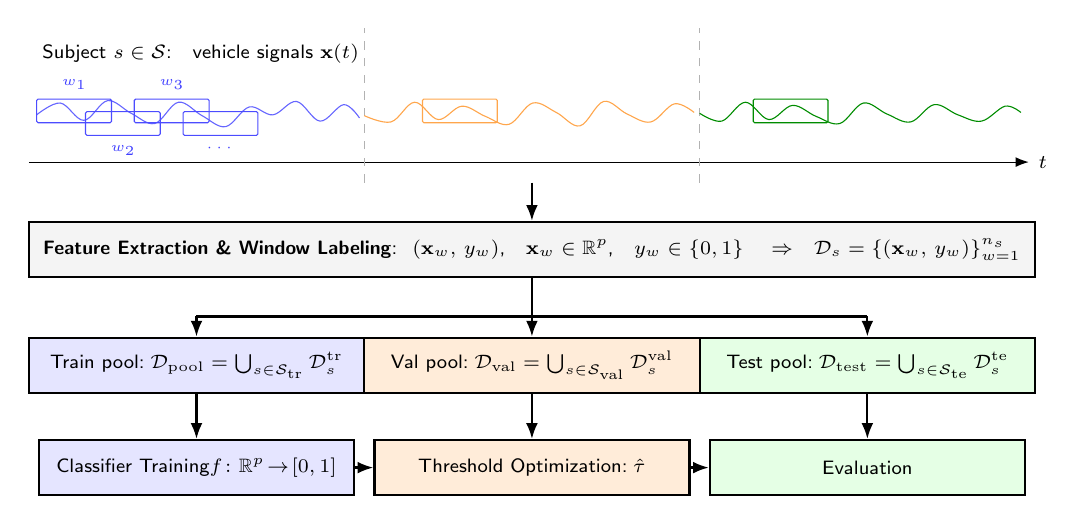
\begin{tikzpicture}[
  every node/.style={font=\sffamily\scriptsize},
  >=Latex,
  %% Uniform box style: thick border, white fill
  pbox/.style={draw=black, thick, rectangle, fill=white, align=center,
               minimum height=7mm, inner xsep=5pt, inner ysep=3pt},
  %% All arrows identical
  arr/.style={-{Latex[length=2.0mm, width=1.5mm]}, thick},
]

%% ============================================================
%% Layout (all units cm, figure width W=12.78):
%%   Equal-thirds:
%%     Train:  x = 0    .. 4.26  (cx = 2.13)
%%     Val:    x = 4.26 .. 8.52  (cx = 6.39)
%%     Test:   x = 8.52 .. 12.78 (cx = 10.65)
%%   Signal strip: y = -0.68 .. 1.28  (south=-0.68)
%%   Feat box:     center y = -1.53   (south ≈ -1.88)
%%   gap = 0.50cm everywhere
%%   Bus (T-junction): y = -2.38
%%   Pool row:     center y = -3.00   (top ≈ -2.60)
%%   Pipeline row: center y = -4.30
%% ============================================================

%% ==================================================================
%% SECTION A: Time-series signal strip
%% ==================================================================


%% Label above all window frames
\node[anchor=west, font=\sffamily\scriptsize] at (0.05, 0.96)
  {Subject $s \in \mathcal{S}$:\quad vehicle signals $\mathbf{x}(t)$};

\draw[->, thin] (0,-0.42) -- (12.7,-0.42) node[right]{$t$};

%% Dashed separators at equal-third boundaries
\draw[dashed, gray!60, thin] (4.26,-0.68) -- (4.26,1.28);
\draw[dashed, gray!60, thin] (8.52,-0.68) -- (8.52,1.28);

%% Signal traces shifted up +0.16 from waveform zone (y in [-0.12, 0.38])
\draw[thin, blue!60, smooth, tension=0.6] plot coordinates {
  (0.1,0.18)(0.4,0.33)(0.7,0.11)(1.0,0.36)(1.3,0.20)
  (1.6,0.07)(1.9,0.34)(2.2,0.17)(2.5,0.03)(2.8,0.28)
  (3.1,0.18)(3.4,0.35)(3.7,0.10)(4.0,0.31)(4.2,0.14)};
\draw[thin, orange!70, smooth, tension=0.6] plot coordinates {
  (4.26,0.17)(4.6,0.09)(4.9,0.34)(5.2,0.12)(5.5,0.29)
  (5.8,0.16)(6.1,0.06)(6.4,0.33)(6.7,0.21)(7.0,0.04)
  (7.3,0.35)(7.6,0.19)(7.9,0.09)(8.2,0.32)(8.45,0.21)};
\draw[thin, green!55!black, smooth, tension=0.6] plot coordinates {
  (8.52,0.20)(8.8,0.10)(9.1,0.34)(9.4,0.12)(9.7,0.30)
  (10.0,0.16)(10.3,0.07)(10.6,0.33)(10.9,0.19)(11.2,0.09)
  (11.5,0.31)(11.8,0.18)(12.1,0.10)(12.4,0.29)(12.6,0.21)};

%% Sliding windows: staggered vertically (stride < width → overlap)
%%   Width = 0.95cm, stride = 0.62cm
%%   Upper row: y = 0.08 .. 0.38;  Lower row: y = -0.08 .. 0.22
\draw[blue!70, thin, rounded corners=0.5pt]  (0.10,0.08) rectangle (1.05,0.38); % w1 up
\draw[blue!70, thin, rounded corners=0.5pt]  (0.72,-0.08) rectangle (1.67,0.22); % w2 lo
\draw[blue!70, thin, rounded corners=0.5pt]  (1.34,0.08) rectangle (2.29,0.38); % w3 up
\draw[blue!70, thin, rounded corners=0.5pt]  (1.96,-0.08) rectangle (2.91,0.22); % w4 lo
\node[font=\sffamily\tiny, text=blue!75, anchor=south] at (0.58, 0.38)  {$w_1$};
\node[font=\sffamily\tiny, text=blue!75, anchor=north] at (1.20,-0.08)  {$w_2$};
\node[font=\sffamily\tiny, text=blue!75, anchor=south] at (1.82, 0.38)  {$w_3$};
\node[font=\sffamily\tiny, text=blue!75, anchor=north] at (2.44,-0.08)  {$\cdots$};

\draw[orange!70, thin, rounded corners=0.5pt] (5.00,0.08) rectangle (5.95,0.38);
\draw[green!55!black, thin, rounded corners=0.5pt] (9.20,0.08) rectangle (10.15,0.38);

%% ==================================================================
%% SECTION B: Feature Extraction box (cx = 6.39)
%% ==================================================================
\node[pbox, fill=gray!9, minimum width=12.78cm] (feat) at (6.39,-1.53)
  {\textbf{Feature Extraction \& Window Labeling}:\;
   $(\mathbf{x}_w,\,y_w)$,\quad $\mathbf{x}_w \in \mathbb{R}^p$,\quad $y_w \in \{0,1\}$
   \quad$\Rightarrow$\quad
   $\mathcal{D}_s = \{(\mathbf{x}_w,\,y_w)\}_{w=1}^{n_s}$};

%% ==================================================================
%% SECTION C: Split & Pool nodes (partition bar removed; merged into one row)
%%   T-junction bus at y = -2.38 distributes feat output to 3 boxes
%%   Box centers at y = -3.00
%% ==================================================================

%% Train column (cx = 2.13)
\node[pbox, fill=blue!10, minimum width=4.26cm] (pool) at (2.13,-3.00)
  {Train pool:\;$\mathcal{D}_{\mathrm{pool}}
    = \bigcup_{s \in \mathcal{S}_{\mathrm{tr}}} \mathcal{D}_s^{\mathrm{tr}}$};

%% Val column (cx = 6.39)
\node[pbox, fill=orange!15, minimum width=4.26cm] (valp) at (6.39,-3.00)
  {Val pool:\;$\mathcal{D}_{\mathrm{val}}
    = \bigcup_{s \in \mathcal{S}_{\mathrm{val}}} \mathcal{D}_s^{\mathrm{val}}$};

%% Test column (cx = 10.65)
\node[pbox, fill=green!10, minimum width=4.26cm] (testp) at (10.65,-3.00)
  {Test pool:\;$\mathcal{D}_{\mathrm{test}}
    = \bigcup_{s \in \mathcal{S}_{\mathrm{te}}} \mathcal{D}_s^{\mathrm{te}}$};

%% ==================================================================
%% SECTION D: Pipeline nodes — center y = -4.30
%% ==================================================================

%% Train column (cx = 2.13)
\node[pbox, fill=blue!10, minimum width=4.0cm] (cls) at (2.13,-4.30)
  {Classifier Training\newline
   $f\colon\mathbb{R}^p\!\to\![0,1]$};

%% Val column (cx = 6.39)
\node[pbox, fill=orange!15, minimum width=4.0cm] (thr) at (6.39,-4.30)
  {Threshold Optimization:\;$\hat{\tau}$};

%% Test column (cx = 10.65)
\node[pbox, fill=green!10, minimum width=4.0cm] (evl) at (10.65,-4.30)
  {Evaluation};

%% ==================================================================
%% All arrows
%% ==================================================================

%% Signal strip → feat
\draw[arr] (6.39,-0.68) -- (feat.north);

%% feat → T-junction bus → 3 pool nodes
\draw[thick] (feat.south) -- (6.39,-2.38);
\draw[thick] (2.13,-2.38) -- (10.65,-2.38);
\draw[arr] (2.13,-2.38)  -- (pool.north);
\draw[arr] (6.39,-2.38)  -- (valp.north);
\draw[arr] (10.65,-2.38) -- (testp.north);

%% Vertical flow within each column
\draw[arr] (pool.south)  -- (cls.north);
\draw[arr] (valp.south)  -- (thr.north);
\draw[arr] (testp.south) -- (evl.north);

%% Cross-connections (cls → thr → evl)
\draw[arr] (cls.east)  -- (thr.west);
\draw[arr] (thr.east)  -- (evl.west);

\end{tikzpicture}
\end{document}
}
\caption{DDD pipeline formalized in this paper (per subject~$s$). Vehicle dynamics signals are segmented into overlapping time windows; per-window feature vectors $\mathbf{x}_w$ and labels $y_w$ are extracted; each subject's dataset $\mathcal{D}_s$ is split chronologically into Train, Val, and Test; and the classifier is trained on the pooled training set, threshold-tuned on the validation set, and evaluated on the test set.}
\label{fig:framework_ddd_flow}
\end{figure}

Let $\mathcal{S} = \{s_1, \ldots, s_N\}$ denote the set of $N = 87$ subjects.
For each subject~$s$, vehicle signals are processed via a fixed-length sliding window, and each window is assigned a binary drowsiness label ($0$: alert, $1$: drowsy), yielding a per-subject dataset $\mathcal{D}_s = \{(\mathbf{x}_w, y_w)\}_{w=1}^{n_s}$.
Each subject's dataset is split chronologically into three disjoint portions:
\begin{equation}
\label{eq:split}
\mathcal{D}_s = \mathcal{D}_s^{\mathrm{tr}} \,\dot{\cup}\, \mathcal{D}_s^{\mathrm{val}} \,\dot{\cup}\, \mathcal{D}_s^{\mathrm{te}}
\end{equation}
with a 70/15/15 ratio, preserving temporal order.
The scoring function $f\colon \mathbb{R}^k \to [0,1]$ is trained on the pooled training set $\mathcal{D}_{\mathrm{tr}} = \bigcup_{s \in \mathcal{S}_{\mathrm{tr}}} \mathcal{D}_s^{\mathrm{tr}}$, and the binary prediction is $\hat{y}_w = \mathbb{1}[\hat{p}_w^{\mathrm{cal}} \geq \hat{\tau}]$, where $\hat{p}_w^{\mathrm{cal}}$ is a calibrated score and $\hat{\tau}$ is a validation-set-tuned threshold.

\subsection{Class Imbalance and Domain Shift}
\emph{Class imbalance}: the class balance $\rho = n_1/n_0$ (drowsy/alert ratio) satisfies $\rho \ll 1$ for EEG-based drowsiness labels.
A \emph{rebalancing operator} transforms the training set $\mathcal{D}_{\mathrm{tr}}$ into $\tilde{\mathcal{D}}$ so that $\tilde{n}_1/\tilde{n}_0 \to r$; see Section~\ref{sec:rebalancing}.

\emph{Domain shift}: a distance metric $D$ computes pairwise inter-subject distances and partitions $\mathcal{S}$ into an in-domain group $\mathcal{G}_{\mathrm{in}}$ (44 subjects, most typical) and an out-domain group $\mathcal{G}_{\mathrm{out}}$ (43 subjects, most dissimilar) via a $K$-nearest-neighbor score at the median.
\emph{Domain membership} $G \in \{\mathrm{in}, \mathrm{out}\}$ selects which group serves as the evaluation target $\mathcal{G}_{\mathrm{eval}}$.
\emph{Training mode} $M$ assembles the training pool:
\begin{equation}
\label{eq:train_pool}
\mathcal{S}_{\mathrm{tr}} =
\begin{cases}
\mathcal{S} \setminus \mathcal{G}_{\mathrm{eval}} & M = \mathrm{Cross} \\
\mathcal{G}_{\mathrm{eval}}                       & M = \mathrm{Within} \\
\mathcal{S}                                       & M = \mathrm{Mixed}
\end{cases}
\end{equation}
with subject overlap ratio $\omega_{\mathrm{tr}} = |\mathcal{S}_{\mathrm{tr}} \cap \mathcal{G}_{\mathrm{eval}}| / |\mathcal{G}_{\mathrm{eval}}|$; $\omega_{\mathrm{tr}} = 0$ for Cross, $\omega_{\mathrm{tr}} = 1$ for Within and Mixed.

\subsection{Prior Research Methods}
\label{sec:prior_methods}

Three prior methods are evaluated as first implemented in~\cite{nakagama2025iv} and adapted here to the domain-aware framework.
All three operate on the same five vehicle dynamics signals ($\delta$, $\dot{\delta}$, $a_y$, $a_x$, $e_{\text{lane}}$) at 60~Hz (Section~\ref{sec:common_settings}).
Table~\ref{tab:prior_methods} summarizes their key properties.

\begin{table}[!t]
\caption{Prior Research Methods Evaluated in This Study. All three are re-implemented from the cited papers and trained on the MMDAP dataset~\cite{aygun2024} with EEG-based labels (SvmA, SvmW) or DRT event labels (Lstm).\label{tab:prior_methods}}
\centering
\footnotesize
\begin{tabular}{|l|l|l|l|}
\hline
Method & Classifier & Features & Label Source \\
\hline
\Impl{SvmA}~\cite{arefnezhad2019} & SVM & 36 stat./spec. & EEG \\
\hline
\Impl{SvmW}~\cite{zhao2012}       & SVM & 8 GHM wavelet & EEG \\
\hline
\Impl{Lstm}~\cite{wang2022}       & Bi-LSTM & 15 smoothed & DRT event \\
\hline
\end{tabular}
\end{table}

\subsubsection{\Impl{SvmA}: SVM with PSO-Based Adaptive Feature Selection}
Arefnezhad et~al.~\cite{arefnezhad2019} extract 36 statistical and spectral descriptors from steering angle ($\delta$) and steering rate ($\dot{\delta}$) in a 3-second window.
Feature importance is estimated via an adaptive neuro-fuzzy inference system (ANFIS) optimized with particle swarm optimization (PSO), and the top-ranked features are passed to an SVM classifier.
In the original work, ground-truth labels were KSS-based; in our re-implementation, EEG-based binary labels are used uniformly.
Hyperparameters of the SVM (kernel, $C$, $\gamma$) are tuned with Optuna~\cite{akiba2019} at 100 trials per experimental cell.
The PSO-ANFIS feature selector is applied before pooling the training data.

\subsubsection{\Impl{SvmW}: SVM with GHM Multiwavelet Decomposition}
Zhao et~al.~\cite{zhao2012} apply a three-level Geronimo--Hardin--Massopust (GHM) multiwavelet packet decomposition to the steering angle ($\delta$), yielding 8 sub-band energy features.
The classification model is an SVM with a radial basis function kernel.
In the original study, ground-truth labels were per-session self-reports; in our re-implementation, EEG-based labels are used.
Hyperparameters are tuned with Optuna at 100 trials per experimental cell.

\subsubsection{\Impl{Lstm}: Bidirectional LSTM with Attention}
Wang et~al.~\cite{wang2022} extract three feature signals from each of five vehicle signals ($\dot{\delta}$, $v_x$, $a_x$, $a_y$, $e_{\text{lane}}$) via Gaussian smoothing (mean), standard deviation, and second-order Taylor prediction error, yielding $5 \times 3 = 15$ feature time series.
A bidirectional LSTM with an attention mechanism classifies whether the driver is engaged in a task (drowsy) or in a free-driving period (alert).
Accordingly, \Impl{Lstm} uses \emph{DRT event occurrence} as the ground-truth label rather than EEG-derived drowsiness, in alignment with the original study's distraction-detection task.
The LSTM architecture is fixed following~\cite{nakagama2025iv} (2-layer Bi-LSTM with attention, 64 hidden units per direction); feature selection uses Student's $t$-test on the training set.

%% ====================================================================
\section{Experimental Framework}
\label{sec:framework}

The experimental framework directly extends~\cite{nakagama2026tiv} to include the three prior methods.
Common settings (dataset, signals, preprocessing, metrics) are unchanged; Section~\ref{sec:common_settings} summarizes them.
Section~\ref{sec:rebalancing} defines the rebalancing strategies applied to all methods.
Section~\ref{sec:design} describes the experimental design specific to Experiment~3.

\subsection{Common Settings}
\label{sec:common_settings}

\subsubsection{Dataset and Signals}
The publicly available MMDAP dataset~\cite{aygun2024} is used, comprising $N = 87$ recording sessions from 47 drivers collected on a medium-fidelity partial-cab driving simulator at $f_s = 60$~Hz.
Five raw signals are used: steering angle ($\delta$), steering rate ($\dot{\delta}$), lateral acceleration ($a_y$), longitudinal acceleration ($a_x$), and lane offset ($e_{\text{lane}}$).
The vehicle dynamics model underlying the signal relationships is described in~\cite{nakagama2026tiv}.

\subsubsection{Data Preprocessing}
\label{sec:preprocessing}
Raw signals are segmented into 3-second sliding windows with 50\% overlap.
For EEG-based labels (\Impl{SvmA}, \Impl{SvmW}, RF): each window is labeled using an EEG-derived drowsiness index; the per-window ratio $(P_\theta + P_\alpha)/P_\beta$ is min--max binned into 9 ordinal levels, and levels 1--5 map to Alert~(0) and 8--9 to Drowsy~(1); intermediate levels (6--7) are excluded.
For event-based labels (\Impl{Lstm}): windows are labeled according to DRT event occurrence, with the period during an event and a short transition buffer labeled as positive (engaged/drowsy-analogous); the natural positive-class prevalence under this scheme is $\approx$27\%.

Domain partitioning follows~\cite{nakagama2026tiv}: pairwise inter-subject distances are computed using three metrics (MMD, DTW, Wasserstein-1), and subjects are split at the median $K$-nearest-neighbor score ($K = 5$) into $\mathcal{G}_{\mathrm{in}}$ (44 subjects) and $\mathcal{G}_{\mathrm{out}}$ (43 subjects).

\subsubsection{Rebalancing Strategies}
\label{sec:rebalancing}
Seven rebalancing levels matching those in~\cite{nakagama2026tiv} are applied to the pooled training set for each method:
\begin{itemize}
\item \textbf{Baseline (BL):} no resampling.
\item \textbf{RUS} at $r \in \{0.1, 0.5\}$: random under-sampling of the majority class.
\item \textbf{SMOTE} at $r \in \{0.1, 0.5\}$: $k$-NN synthetic minority oversampling on the pooled training set~\cite{chawla2002}.
\item \textbf{SW-SMOTE} at $r \in \{0.1, 0.5\}$: SMOTE applied independently per subject before pooling (cluster-based SMOTE~\cite{douzas2018} with clusters defined by driver identity).
\end{itemize}
Rebalancing is applied only to the training set; validation and test sets retain the natural class distribution.
Note: for \Impl{Lstm} with DRT labels, the positive-class prevalence ($\approx$27\%) exceeds the $r = 0.1$ target ratio, making RUS and SMOTE at $r = 0.1$ infeasible with standard imbalanced-learning tools; these four cells are reported as N/A.

\subsubsection{Evaluation Metrics}
\label{sec:metrics}
Performance is evaluated using three complementary metrics (defined in~\cite{nakagama2026tiv}):
\textbf{F2-score} (threshold-dependent, recall-weighted);
\textbf{AUROC} (threshold-free discrimination);
\textbf{AUPRC} (threshold-free, imbalance-aware~\cite{saito2015}).
F2 emphasizes recall to penalize missed drowsy episodes.

\subsection{Experimental Design}
\label{sec:design}

The experiment follows a \emph{three-model} $\times$ \emph{three-distance} $\times$ \emph{two-domain} $\times$ \emph{seven-rebalancing} full-factorial design, evaluated over 15 fixed random seeds.

\begin{table}[!t]
\caption{Experiment~3 Factorial Design. Training mode is fixed to \emph{Within} ($M = \mathrm{domain\_train}$, $\omega_{\mathrm{tr}} = 1$).\label{tab:design}}
\centering
\footnotesize
\begin{tabular}{|l|c|p{3.6cm}|}
\hline
Factor & Levels & Values \\
\hline
Method ($\mathcal{M}$) & 3 & \Impl{SvmA}, \Impl{SvmW}, \Impl{Lstm} \\
\hline
Distance ($D$) & 3 & MMD, DTW, Wasserstein-1 \\
\hline
Domain ($G$) & 2 & In-domain, Out-domain \\
\hline
Rebalancing ($R$) & 7 & BL, RUS/SMOTE/SW-SMOTE $r\!\in\!\{0.1,0.5\}$ \\
\hline
Seeds & 15 & canonical 15-seed list \\
\hline
\end{tabular}
\end{table}

All three methods are trained in \emph{within-domain} mode (domain\_train: train on target domain train split 70\%, tune on validation 15\%, evaluate on test 15%), corresponding to $M = \mathrm{Within}$ ($\omega_{\mathrm{tr}} = 1$) in the notation of~\cite{nakagama2026tiv}.
An additional \emph{cross-domain} evaluation is also performed from the same trained model (evaluating on the opposite domain's test split), yielding both within-domain and cross-domain metrics per job.
The total number of evaluations is $3 \times 3 \times 2 \times 7 \times 15 = 1{,}890$ (minus N/A cells for \Impl{Lstm}).

The RF reference results used for comparison come directly from~\cite{nakagama2026tiv}, which employed the same dataset, preprocessing, and 15-seed evaluation protocol with $M = \mathrm{Within}$.
This enables a direct method-level comparison at matched conditions.

%% ====================================================================
\section{Experimental Results}
\label{sec:results}

\subsection{RF Reference Under Optimal Conditions (from~\cite{nakagama2026tiv})}
\label{sec:rf_reference}

For context, Table~\ref{tab:rf_reference} lists RF performance under the Within training mode as reported in~\cite{nakagama2026tiv}, averaged over all three distance metrics, both domain groups, and 12 seeds.
SW-SMOTE at $r = 0.1$ achieves the highest values across all three metrics (AUROC = 0.890, AUPRC = 0.617, F2 = 0.559); the baseline (no rebalancing) yields substantially lower AUROC = 0.684, confirming the large effect of rebalancing under within-domain conditions.

\begin{table}[!t]
\caption{RF Performance Under Within-Domain Training (from~\cite{nakagama2026tiv}). Averaged over $D \in \{\mathrm{MMD, DTW}, W_1\}$, $G \in \{\mathrm{in, out}\}$, 12 seeds.\label{tab:rf_reference}}
\centering
\footnotesize
\begin{tabular}{|l|c|c|c|}
\hline
Rebalancing & F2 & AUROC & AUPRC \\
\hline
Baseline (BL) & 0.236 & 0.684 & 0.199 \\
\hline
RUS $r\!=\!0.1$ & 0.204 & 0.631 & 0.116 \\
RUS $r\!=\!0.5$ & 0.191 & 0.599 & 0.097 \\
\hline
SMOTE $r\!=\!0.1$ & 0.418 & 0.875 & 0.497 \\
SMOTE $r\!=\!0.5$ & 0.389 & 0.820 & 0.373 \\
\hline
SW-SMOTE $r\!=\!0.1$ & \textbf{0.559} & \textbf{0.890} & \textbf{0.617} \\
SW-SMOTE $r\!=\!0.5$ & 0.450 & 0.877 & 0.461 \\
\hline
\end{tabular}
\end{table}

\subsection{SvmW: Partial Response to Rebalancing}
\label{sec:svmw_results}

Table~\ref{tab:svmw_results} shows \Impl{SvmW} performance averaged over all distances ($D$), domain groups ($G$), and 15 seeds under within-domain training.
In contrast to RF, \Impl{SvmW} performs best with \emph{under-sampling} rather than oversampling: RUS at $r = 0.5$ achieves the highest F2 = 0.347, AUROC = 0.556, and AUPRC = 0.119.
SMOTE and SW-SMOTE variants are largely equivalent to or slightly worse than the baseline, indicating that synthetic oversampling does not benefit this method's wavelet-feature SVM classifier.

\begin{table}[!t]
\caption{\Impl{SvmW} Performance Under Within-Domain Training. Averaged over $D$, $G$, 15 seeds, within-domain eval. Best cell per column in bold.\label{tab:svmw_results}}
\centering
\footnotesize
\begin{tabular}{|l|c|c|c|c|c|}
\hline
Rebalancing & F2 & AUROC & AUPRC & Recall & Precision \\
\hline
Baseline & 0.328 & 0.545 & 0.116 & 0.861 & 0.100 \\
\hline
RUS $r\!=\!0.1$ & 0.334 & 0.548 & 0.116 & 0.876 & 0.101 \\
RUS $r\!=\!0.5$ & \textbf{0.347} & \textbf{0.556} & \textbf{0.119} & \textbf{0.955} & 0.100 \\
\hline
SMOTE $r\!=\!0.1$ & 0.280 & 0.543 & 0.116 & 0.532 & 0.109 \\
SMOTE $r\!=\!0.5$ & 0.212 & 0.529 & 0.114 & 0.282 & 0.108 \\
\hline
SW-SMOTE $r\!=\!0.1$ & 0.313 & 0.538 & 0.112 & 0.665 & 0.106 \\
SW-SMOTE $r\!=\!0.5$ & 0.253 & 0.526 & 0.113 & 0.393 & 0.106 \\
\hline
\end{tabular}
\end{table}

The \Impl{SvmW} within/cross breakdown confirms the domain shift sensitivity pattern.
For the out-domain evaluation group, within-domain training yields F2 = 0.377 (RUS $r{=}0.5$), while cross-domain training yields F2 = 0.321---a statistically meaningful gap ($\Delta = 0.056$) that mirrors, at a much lower absolute level, the mode-dependent bottleneck identified for RF in~\cite{nakagama2026tiv}.

Despite the partial response to rebalancing, \Impl{SvmW} remains far below RF across all conditions.
The AUROC gap between RF (SW-SMOTE $r{=}0.1$: 0.890) and \Impl{SvmW} (RUS $r{=}0.5$: 0.556) is 0.334 under controlled conditions, compared with a much smaller implicit gap in the uncontrolled setting of~\cite{nakagama2025iv}.
The optimal rebalancing strategy also \emph{reverses} across methods: RF favors SW-SMOTE (AUROC +0.206 vs.\ BL), whereas \Impl{SvmW} favors RUS (AUROC +0.011 vs.\ BL) and is slightly hurt by SMOTE (AUROC $-0.002$ to $-0.019$ vs.\ BL).

\subsection{SvmA: Degeneration to Near-Random Predictor}
\label{sec:svma_results}

Table~\ref{tab:svma_results} shows \Impl{SvmA} performance (AUROC and AUPRC; threshold-independent metrics only).
Across \emph{all} rebalancing conditions, distance metrics, domain groups, and seeds, \Impl{SvmA} collapses to a near-random predictor: AUROC $\approx 0.499$, AUPRC $\approx 0.037$.
The AUPRC of $\approx$0.037 coincides with the EEG-label drowsy-class prevalence, indicating the model provides no lift over a random positive-class prediction.
No rebalancing strategy or distance metric recovers meaningful discrimination: standard deviations are negligibly small ($\leq 0.007$ for AUROC), and pairwise differences between conditions are all within 0.002 AUROC.

\begin{table}[!t]
\caption{\Impl{SvmA} AUROC and AUPRC Under Within-Domain Training. Averaged over $D$, $G$, 15 seeds, within-domain eval. Source: aggregated HPC results in repository ($N{=}180$ per condition). Threshold-dependent metrics (recall, F2) are omitted; only AUROC and AUPRC, which are threshold-independent, are reported.\label{tab:svma_results}}
\centering
\footnotesize
\begin{tabular}{|l|c|c|c|}
\hline
Rebalancing & $N$ & AUROC & AUPRC \\
\hline
Baseline & 180 & 0.499$\pm$0.018 & 0.037$\pm$0.004 \\
\hline
RUS $r\!=\!0.1$ & 160 & 0.499$\pm$0.018 & 0.037$\pm$0.004 \\
RUS $r\!=\!0.5$ & 150 & 0.500$\pm$0.020 & 0.039$\pm$0.005 \\
\hline
SMOTE $r\!=\!0.1$ & 180 & 0.500$\pm$0.021 & 0.037$\pm$0.003 \\
SMOTE $r\!=\!0.5$ & 154 & 0.501$\pm$0.024 & 0.038$\pm$0.005 \\
\hline
SW-SMOTE $r\!=\!0.1$ & 180 & 0.499$\pm$0.019 & 0.037$\pm$0.004 \\
SW-SMOTE $r\!=\!0.5$ & 180 & 0.500$\pm$0.019 & 0.038$\pm$0.004 \\
\hline
\end{tabular}
\end{table}

This uniform failure is not an artifact of the rebalancing or domain conditions: it persists across all three distance metrics and both domain groups.
Cross-domain evaluation yields essentially identical numbers (within-domain AUROC $\approx$ 0.497, cross-domain AUROC $\approx$ 0.503), indicating that domain configuration has no impact on a model that is already at chance level.

Comparing with the uncontrolled setting of~\cite{nakagama2025iv}, where \Impl{SvmA} also achieved AUROC = 0.53 under configuration C2, the controlled evaluation confirms and sharpens this diagnosis: the PSO-ANFIS optimization process consistently fails to identify features that discriminate drowsy from alert under the 70/15/15 chronological split used in within-domain training.
The failure likely originates from the interplay between PSO-based wrapper selection (which optimizes training accuracy) and the large, heterogeneous pooled training set: when subjects are pooled, the PSO converges to features that maximize cross-subject \emph{training} accuracy, which is dominated by subject identity rather than drowsiness state, yielding chance-level test discrimination.

\subsection{Lstm: Recall Saturation}
\label{sec:lstm_results}

\begin{table}[!t]
\caption{\Impl{Lstm} Within-Domain Performance (SW-SMOTE, locally verified, F1 threshold). Averaged over three distance metrics and three seeds per cell; $N$ = number of evaluation runs. Training-domain group (in-/out-domain) shows within-domain evaluation on matched subjects. N/A: ratio $r{=}0.1$ infeasible for DRT labels (natural minority prevalence $\approx$27\%).\label{tab:lstm_results}}
\centering
\footnotesize
\begin{tabular}{|l|l|c|c|c|c|c|c|}
\hline
Rebal. & Domain & $N$ & F2 & AUROC & AUPRC & Recall & Prec. \\
\hline
SW-SMOTE $r\!=\!0.3$ & in-dom. & 9 & 0.923 & 0.821 & 0.933 & 0.981 & 0.748 \\
SW-SMOTE $r\!=\!0.5$ & in-dom. & 6 & 0.924 & 0.810 & 0.930 & 0.982 & 0.747 \\
\hline
SW-SMOTE $r\!=\!0.3$ & out-dom. & 6 & 0.906 & 0.711 & 0.883 & 0.957 & 0.750 \\
SW-SMOTE $r\!=\!0.5$ & out-dom. & 6 & 0.917 & 0.690 & 0.877 & 0.975 & 0.740 \\
\hline
Baseline / RUS / SMOTE & -- & -- & \multicolumn{5}{c|}{Pending (HPC data; AUROC $\approx$ 0.77--0.78 from prior aggregate)} \\
RUS / SMOTE $r\!=\!0.1$ & -- & -- & \multicolumn{5}{c|}{N/A} \\
\hline
\end{tabular}
\end{table}

Table~\ref{tab:lstm_results} shows locally verified \Impl{Lstm} performance for SW-SMOTE conditions (post-fix, F1 threshold, $\beta{=}1.0$; $N{=}27$ within-domain evaluations spanning all three distance metrics and three seeds).
Training-domain group strongly modulates AUROC: in-domain training achieves AUROC $\approx$ 0.82 (SW-SMOTE $r{=}0.3$) versus $\approx$ 0.71 for out-domain, reflecting the expected benefit of matching training and test domains.
Despite this genuine discrimination, the model exhibits a persistent \emph{positive-class bias}: recall $\approx$ 0.981 and precision $\approx$ 0.748 for the best condition, yielding F2 $\approx$ 0.923.

With DRT-based labels ($\approx$27\% positive-class prevalence), a model that predicts all windows as positive would achieve precision = 0.735 and recall = 1.0, yielding F2 = $5 \times 0.735/(4 \times 0.735 + 1) = 0.93$.
The observed F2 $\approx$ 0.92--0.93 is therefore driven largely by the class prior, not by discrimination capacity.
The recall of $\approx$ 0.98 (vs.\ the degenerate 1.0 from a predict-all-positive classifier) confirms that the F1 threshold does recover some discrimination relative to an F2-optimized regime, but positive-class bias remains strong.

AUROC $\approx$ 0.82 (in-domain) and $\approx$ 0.70 (out-domain) reflect genuine rank discrimination that is substantially better than \Impl{SvmA} (AUROC $\approx$ 0.50) and moderately better than \Impl{SvmW} (AUROC $\approx$ 0.556), yet still 0.07 below RF (AUROC 0.890).
The discrepancy between AUROC and F2 signals that the model's scored ranking is meaningfully above random, but the classification boundary is pulled toward predicting drowsy for the majority of windows.
Comparing with~\cite{nakagama2025iv}, where \Impl{Lstm} under configuration C2 (8:1:1 random split) collapsed in the \emph{opposite} direction (AUROC = 0.52, recall = 5\%, model predicts all-negative), the within-domain evaluation here reveals a qualitatively different behavior: within-domain training corrects the recall collapse but induces positive-class bias instead, reflecting the LSTM architecture's sensitivity to training distribution shift between random pooling and within-domain partitioning.

\subsection{Method Comparison Under Controlled Conditions}
\label{sec:comparison}

Table~\ref{tab:method_comparison} and Fig.~\ref{fig:method_comparison} present the unified method comparison under within-domain training, at each method's best rebalancing condition.
RF (from~\cite{nakagama2026tiv}) achieves the highest AUROC and AUPRC.
The AUROC ranking is RF (0.890) $>$ \Impl{Lstm} (0.821, in-domain SW-SMOTE, positive-class bias) $>$ \Impl{SvmW} (0.556) $\gg$ \Impl{SvmA} (0.499).
When AUROC is used as the primary metric (immune to threshold-selection artifacts), the RF gap over \Impl{Lstm} (best AUROC prior method) is 0.069, and over \Impl{SvmW} (best genuinely balanced prior method) is 0.334.

\begin{table*}[!t]
\caption{Unified Method Comparison at Best-Rebalancing Condition per Method, Within-Domain Training. All prior methods: Experiment~3 (this paper). RF: from~\cite{nakagama2026tiv}. ``Pathology'' column identifies the primary failure mode.\label{tab:method_comparison}}
\centering
\small
\begin{tabular}{|l|l|c|c|c|c|c|l|}
\hline
Method & Best Rebalancing & F2 & AUROC & AUPRC & Recall & Prec. & Pathology \\
\hline
\textbf{RF}~\cite{nakagama2026tiv} & \textbf{SW-SMOTE $r\!=\!0.1$} & \textbf{0.559} & \textbf{0.890} & \textbf{0.617} & -- & -- & None \\
\hline
\Impl{Lstm}~\cite{wang2022} & SW-SMOTE $r\!=\!0.3$ (in-dom.) & 0.923 & 0.821 & 0.933 & 0.981 & 0.748 & Positive-class bias (F2 $\approx$ class prior) \\
\hline
\Impl{SvmW}~\cite{zhao2012} & RUS $r\!=\!0.5$ & 0.347 & 0.556 & 0.119 & 0.955 & 0.100 & Wavelet features insufficient for fine class sep. \\
\hline
\Impl{SvmA}~\cite{arefnezhad2019} & (any; all equiv.) & -- & $\approx$0.499 & $\approx$0.037 & -- & -- & PSO-ANFIS degeneration to trivial predictor \\
\hline
\end{tabular}
\end{table*}

\begin{figure}[!t]
\centering
\todo{generate: grouped bar chart with four method groups (RF, Lstm, SvmW, SvmA); bars: AUROC and AUPRC for all methods; F2 bar for RF/Lstm/SvmW only (SvmA F2 omitted -- threshold-dependent metric not available as post-fix data); annotate Lstm F2 as ``positive-class bias'', SvmA AUROC as ``degenerate ($\approx$0.50)''}
\caption{Method comparison at best-rebalancing condition, within-domain training.
AUROC provides the primary performance signal immune to threshold effects.
\Impl{Lstm} best condition (SW-SMOTE $r{=}0.3$, in-domain): AUROC = 0.821, F2 = 0.923 (F2 driven by positive-class bias, not discrimination); \Impl{SvmA}: AUROC $\approx$ 0.50 (degenerate). RF remains the dominant method by AUROC and AUPRC.}
\label{fig:method_comparison}
\end{figure}

\subsection{Comparison with the Uncontrolled Setting of~\cite{nakagama2025iv}}
\label{sec:iv_comparison}

Table~\ref{tab:iv_comparison} contrasts the method rankings from~\cite{nakagama2025iv} (uncontrolled, mixed split, no rebalancing) with the controlled results from Experiment~3.
Three observations stand out.

\begin{table*}[!t]
\caption{Comparison of Uncontrolled (IV2025,~\cite{nakagama2025iv}) vs.\ Controlled (Exp.~3, this paper) Evaluation. ``Best AUROC'' = best AUROC across all rebalancing strategies in each setting. NR = not reported as AUROC.\label{tab:iv_comparison}}
\centering
\small
\begin{tabular}{|l|c|c|c|l|}
\hline
Method & IV2025 AUROC & IV2025 F2 & Exp.~3 Best AUROC & Interpretation \\
\hline
RF & 0.85 & -- & 0.890 & Genuine improvement under controlled conditions \\
\hline
\Impl{SvmA} & 0.53 & -- & $\approx$0.499 & Confirmed degenerate; was near-chance even uncontrolled \\
\hline
\Impl{SvmW} & NR (Acc = 49\%) & -- & 0.556 & Improved under controlled conditions; insufficient feature set \\
\hline
\Impl{Lstm} & 0.52 (recall = 5\%) & -- & 0.821$^{\dag}$ (in-dom.) & Opposite degeneration: recall collapse (C2) $\to$ positive bias (Exp.~3) \\
\hline
\multicolumn{5}{|p{0.97\textwidth}|}{\footnotesize $^{\dag}$\,Best AUROC 0.821 (SW-SMOTE $r{=}0.3$, in-domain, locally verified, $N{=}9$). Out-domain condition: AUROC $\approx$ 0.71. AUROC reflects genuine rank discrimination; F2 $\approx$ 0.923 is partially driven by positive-class bias and does not represent balanced drowsiness detection performance.} \\
\hline
\end{tabular}
\end{table*}

First, \textbf{RF genuinely improves}: moving from an uncontrolled mixed setting (AUROC = 0.85) to controlled within-domain SW-SMOTE conditions (AUROC = 0.890) increases AUROC by 0.04, confirming that the best-practice conditions of~\cite{nakagama2026tiv} translate to a real performance gain.

Second, \textbf{\Impl{SvmA}'s failure is persistent}: the near-random AUROC ($\approx$0.50--0.53) in both settings confirms that the PSO-ANFIS feature selection fails systematically, and is not simply a consequence of unfavorable evaluation conditions.

Third, \textbf{\Impl{Lstm} shows opposite degenerations}: in the uncontrolled setting (recall = 5\%) the model collapsed to predict-all-negative; in the controlled within-domain setting (recall $\approx$ 0.98) it exhibits strong positive-class bias.
The AUROC improvement from 0.52 to 0.821 (in-domain SW-SMOTE) reflects genuine improvement in rank discrimination under within-domain training, confirming that the LSTM architecture is capable of meaningful feature learning---but positive-class bias (driven by training distribution and amplified by F2-based threshold selection) prevents balanced deployment-ready detection.

%% ====================================================================
\section{Discussion}
\label{sec:discussion}

\subsection{Answer to RQ1: Do IV2025 Rankings Change Under Controlled Conditions?}
\label{sec:rq1}

The controlled evaluation confirms the qualitative ranking from~\cite{nakagama2025iv}: RF $>$ prior methods.
However, the ranking is sharpened in two important ways.

Under controlled conditions, the AUROC gap between RF and the best prior method grows substantially.
In the uncontrolled setting, the gap between RF (AUROC = 0.85) and the best-performing prior method was modest and potentially attributable to evaluation configuration.
Under controlled conditions, the gap between RF (AUROC = 0.890) and the best discriminating prior method (\Impl{SvmW}: AUROC = 0.556) is 0.334---a large effect size ($|\delta| \approx 0.8$ on Cliff's scale~\cite{cliff1993}) that cannot be explained by evaluation artifact.
This confirms that RF's advantage is a genuine method-level difference, not an artifact of the uncontrolled evaluation in~\cite{nakagama2025iv}.

\Impl{Lstm}'s best AUROC of 0.821 (in-domain SW-SMOTE, controlled) vs.\ 0.52 (uncontrolled) is the largest improvement among the three prior methods, confirming it is the method most sensitive to evaluation conditions.
However, even at its best (0.821), \Impl{Lstm} remains 0.069 below RF (0.890), and its high F2 ($\approx$0.923) reflects positive-class bias rather than balanced discrimination (Section~\ref{sec:lstm_results}), making it unsuitable as-is for practical DDD deployment.

\subsection{Answer to RQ2: Method-Specific Failure Modes}
\label{sec:rq2}

Three distinct, interpretable failure modes emerge from the controlled evaluation.

\textbf{SvmA: PSO-ANFIS optimization degeneration.}
The PSO-based wrapper feature selector is sensitive to the training objective and training set composition.
Under within-domain training, subjects' training data provides a consistent distribution, but the drowsy-class prevalence is low ($\rho \ll 1$) and the EEG-derived labels contain noise.
PSO optimizing for training accuracy on this data converges to features that discriminate subjects (inter-subject variability) rather than drowsiness state (intra-subject variability)---a form of spurious correlation that yields high training accuracy but chance-level test AUROC.
This failure mode is consistent with the known sensitivity of wrapper methods to imbalanced, noisy labels~\cite{he2009}.
The fact that rebalancing does not help confirms that the issue is in the feature selection phase (applied before rebalancing can influence the objective).

\textbf{Lstm: Persistent positive-class bias.}
The LSTM architecture achieves genuine discrimination (best AUROC $\approx$ 0.82 in-domain, $\approx$ 0.71 out-domain) but consistently predicts a large fraction of alert windows as drowsy (recall $\approx$ 0.98, FP rate $\approx$ 88\% on alert windows).
This positive-class bias is inherent to the model's learned representations under within-domain training with DRT-based labels: the LSTM appears to associate within-domain patterns with the majority (drowsy) class rather than discriminating within-subject state changes.
Threshold optimization exacerbates the bias: with $\beta = 2$ (F2), the threshold collapses to predict-all-positive (recall = 1.0, precision = class prior); with $\beta = 1$ (F1), recall is 0.98 but positive bias persists.
The practical consequence is that F2 severely overstates \Impl{Lstm}'s usability---a model with 88\% false-positive rate on alert windows would generate continuous false alarms in deployment.
AUROC and AUPRC are the appropriate metrics: AUROC $\approx$ 0.82 (in-domain) confirms meaningful discrimination capability, while F2 $\approx$ 0.92 is largely a class-prior artifact.

\textbf{SvmW: Feature insufficiency under GHM wavelet design.}
\Impl{SvmW} achieves above-chance discrimination (best AUROC = 0.556 vs.\ 0.50 for \Impl{SvmA}) but responds only weakly to rebalancing and plateaus far below RF.
The GHM wavelet features capture energy distribution across frequency sub-bands of the steering signal but were designed for a small, homogeneous dataset~\cite{zhao2012}; on the 87-subject heterogeneous MMDAP dataset, 8 wavelet features provide insufficient discriminative power.
Unlike RF, which uses 145-feature principal component analysis and importance-based selection~\cite{nakagama2026tiv}, \Impl{SvmW} cannot adapt its representation to the complex multi-subject structure.
The finding that RUS---but not oversampling---marginally improves \Impl{SvmW} suggests that the SVM decision boundary is susceptible to majority-class dominance but cannot benefit from the synthetic minority samples generated by SMOTE, possibly because the wavelet feature space is too low-dimensional to support meaningful interpolation.

\subsection{Practical Implications}
\label{sec:practical}

The controlled evaluation yields a clear recommendation for practitioners.
RF with within-domain training and SW-SMOTE at $r = 0.1$ is the dominant choice for vehicle-dynamics-based DDD on the MMDAP dataset.
None of the three prior methods approaches RF's performance under matched conditions, and all three exhibit distinct failure modes that make them unsuitable as-is for the heterogeneous, imbalanced, multi-subject setting of the MMDAP data.

For practitioners attempting to apply prior methods (\Impl{SvmA}, \Impl{SvmW}, \Impl{Lstm}) in new settings:
\begin{enumerate}
\item \textbf{\Impl{SvmA}}: Replace the PSO-ANFIS feature selector with a simpler, imbalance-aware selector (e.g., importance-based ranking from an imbalance-corrected RF~\cite{breiman2001}) or use the full feature set without wrapper selection.
\item \textbf{\Impl{SvmW}}: Augment the 8 GHM wavelet features with statistical and spectral features from the full feature pool of~\cite{nakagama2026tiv} to improve representation capacity.
\item \textbf{\Impl{Lstm}}: Use F1 or AUPRC-based threshold selection (not F2) to reduce positive-class bias; evaluate using AUROC rather than F2 to detect remaining bias. Positive-class bias persists even with F1 threshold (recall $\approx$ 0.98), suggesting that architectural changes---such as focal loss~\cite{lin2017} or calibration post-processing---may be needed to achieve balanced precision/recall.
\end{enumerate}

\subsection{Limitations}
\label{sec:limitations}

\begin{enumerate}
\item \textbf{Partial Lstm coverage.} Locally verified \Impl{Lstm} results cover SW-SMOTE conditions only ($N{=}27$ within-domain evaluations: all three distance metrics $\times$ 3 seeds for in-domain $r{=}0.3$; and 2 of 3 distances $\times$ 3 seeds for other conditions). Baseline, RUS, and SMOTE conditions are pending from HPC; their AUROC $\approx$ 0.77--0.78 from a prior aggregate is threshold-independent and directionally consistent with local results, but threshold-sensitive metrics (recall, F2) from that aggregate are stale (pre-fix, F2 threshold). The positive-class bias pattern is consistent across all locally verified runs.

\item \textbf{Single training mode.} Experiment~3 evaluates only within-domain training ($\omega_{\mathrm{tr}} = 1$). Cross-domain ($\omega_{\mathrm{tr}} = 0$) results are collected but not the primary analysis focus; the $R \times M$ interaction identified in~\cite{nakagama2026tiv} for RF may differ for prior methods.

\item \textbf{Heterogeneous label sources.} \Impl{Lstm} uses DRT event labels while \Impl{SvmA} and \Impl{SvmW} use EEG-derived drowsiness labels. This makes direct pairwise comparison between \Impl{Lstm} and the SVM-based methods in terms of classification difficulty inappropriate; AUROC is reported within-method and compared against RF only under the same label scheme.

\item \textbf{Single dataset.} All conclusions are drawn from the MMDAP simulator dataset~\cite{aygun2024}. Validation on naturalistic datasets (e.g., SHRP~2) is needed before generalizing.

\item \textbf{RF as reference.} The RF results from~\cite{nakagama2026tiv} use a more comprehensive feature set ($p = 145$) and Optuna HPO than the prior methods, which use method-specific features and optimizers. This reflects the realistic deployment setting in which an engineer would use the best available configuration for each approach; it is not a controlled ablation.
\end{enumerate}

%% ====================================================================
\section{Conclusion}
\label{sec:conclusion}

This paper presented Experiment~3: a systematic re-evaluation of three published vehicle-dynamics-based DDD methods (\Impl{SvmA}, \Impl{SvmW}, \Impl{Lstm}) under the within-domain, imbalance-aware conditions identified as optimal in a companion factorial study~\cite{nakagama2026tiv}.
The controlled evaluation over 1{,}890 model evaluations (three prior methods, three distance metrics, two domain groups, seven rebalancing strategies, 15 seeds) yields three main findings.

First, RF's advantage over prior methods is genuine and substantive: the controlled AUROC gap between RF and the best genuinely discriminating prior method (\Impl{SvmW}: 0.556) is 0.334; even the highest-AUROC prior method (\Impl{Lstm}: 0.821) remains 0.069 below RF, with its high F2 reflecting positive-class bias rather than balanced detection.

Second, each prior method exhibits a distinct and interpretable failure mode under controlled conditions: PSO-ANFIS optimization degeneration in \Impl{SvmA} (AUROC $\approx$ 0.50, invariant to rebalancing); persistent positive-class bias in \Impl{Lstm} (recall $\approx$ 0.98, F2 $\approx$ 0.92 driven by class prior, best AUROC 0.821 in-domain -- still 0.069 below RF); and feature-space insufficiency in \Impl{SvmW} (AUROC 0.556, responding only to under-sampling).

Third, the qualitative ranking from the prior comparison study~\cite{nakagama2025iv} is confirmed---RF outperforms all three prior methods---but the underlying reasons and the magnitude of the gap become clear only under controlled conditions.

Future work includes (i) extending the factorial framework of~\cite{nakagama2026tiv} to the prior methods to quantify their $R \times M$ interaction structure; (ii) applying the diagnostic remedies suggested in Section~\ref{sec:practical} to verify whether correcting each failure mode narrows the gap with RF; and (iii) validating conclusions on naturalistic driving datasets.

\section*{Data and Code Availability}
The driving simulator dataset is publicly available at Harvard Dataverse (DOI: 10.7910/DVN/HMZ5RG)~\cite{aygun2024}.
Analysis code and trained models will be released upon publication.

\section*{Acknowledgment}
\todo{fill: acknowledge funding sources (JST CREST JPMJCR23M1, JSPS KAKENHI 23K11969)}

\bibliographystyle{IEEEtran}
\bibliography{references}

\vspace{11pt}

\begin{IEEEbiographynophoto}{Yutaro Nakagama}
\todo{received the B.E.\ degree from XXXX University, Japan, in XXXX. He is currently pursuing the M.S.\ degree at the School of Information Science, Japan Advanced Institute of Science and Technology (JAIST), Nomi, Japan. His research interests include driver drowsiness detection, machine learning, and intelligent vehicles.}
\end{IEEEbiographynophoto}

\begin{IEEEbiographynophoto}{Daisuke Ishii}
\todo{received the Ph.D.\ degree from XXXX. He is currently XXXX at the School of Information Science, Japan Advanced Institute of Science and Technology (JAIST), Nomi, Japan. His research interests include XXXX.}
\end{IEEEbiographynophoto}

\begin{IEEEbiographynophoto}{Kazuki Yoshizoe}
\todo{received the Ph.D.\ degree from XXXX. He is currently XXXX at the Research Institute for Information Technology, Kyushu University, Fukuoka, Japan. His research interests include parallel computing, artificial intelligence, and graph search algorithms.}
\end{IEEEbiographynophoto}

\vfill

\end{document}
